\chapter{Bunyi di Sekitar Kita}\label{ch:g3:sound-around-us}

Dendangkan lagu kesukaanmu --- dan selagi mendendang, letakkan dua
jari pelan-pelan di depan tenggorokanmu. Terasa getarnya? Kamu baru
saja menyentuh \omterm{def:g3:sound-around-us:sound}{bunyi} di tempat kelahirannya. Setiap suara, setiap
gendang, setiap pintu yang berderit membuat \omterm{def:g3:sound-around-us:sound}{bunyinya} dengan cara yang
persis sama, dan bab ini pergi memburu tipuannya.

\section{Tempat bunyi lahir}

\begin{definition}[Getaran]\label{def:g3:sound-around-us:vibration}
Sebuah \emph{getaran}\index{getaran} adalah gemetar yang sangat cepat
--- gerakan bolak-balik yang berulang berkali-kali tiap sekon, sering
terlalu cepat untuk diikuti mata. Senar gitar yang dipetik bergetar:
kamu hanya melihat bayangan kabur, tetapi ujung jarimu merasakan
dengungnya.
\end{definition}

\begin{definition}[Bunyi]\label{def:g3:sound-around-us:sound}
Sebuah \emph{bunyi}\index{bunyi} adalah apa yang kita dengar ketika
sesuatu bergetar dan \omterm{def:g3:sound-around-us:vibration}{getarannya} merambat melalui \omterm{def:g2:air-around-us:air}{udara} sampai ke
telinga kita. Benda yang bergetar itu adalah \emph{sumber} bunyinya
--- senar, kulit gendang, lonceng, atau tenggorokanmu sendiri.
\end{definition}

\begin{method}[Membuat beras menari]\label{met:g3:sound-around-us:rice}
Untuk \emph{melihat} sebuah \omterm{def:g3:sound-around-us:sound}{bunyi} lahir:
\begin{enumerate}
  \item taburkan beberapa butir beras di atas kulit gendang (atau di
        atas tutup plastik sebuah kaleng, atau kulit balon yang
        diregangkan);
  \item ketuk kulitnya dekat butiran itu --- bum: butirannya
        melompat!
  \item sekarang cukup \emph{berteriaklah} ke arah kulitnya dari
        jarak sangat dekat: butirannya bergetar lagi, tanpa disentuh.
\end{enumerate}
Kulit itu bergetar setiap kali ia berbunyi --- dan bahkan \omterm{def:g3:sound-around-us:sound}{bunyi} yang
datang dari mulutmu pun membuatnya bergetar.
\end{method}

\begin{omfigure}
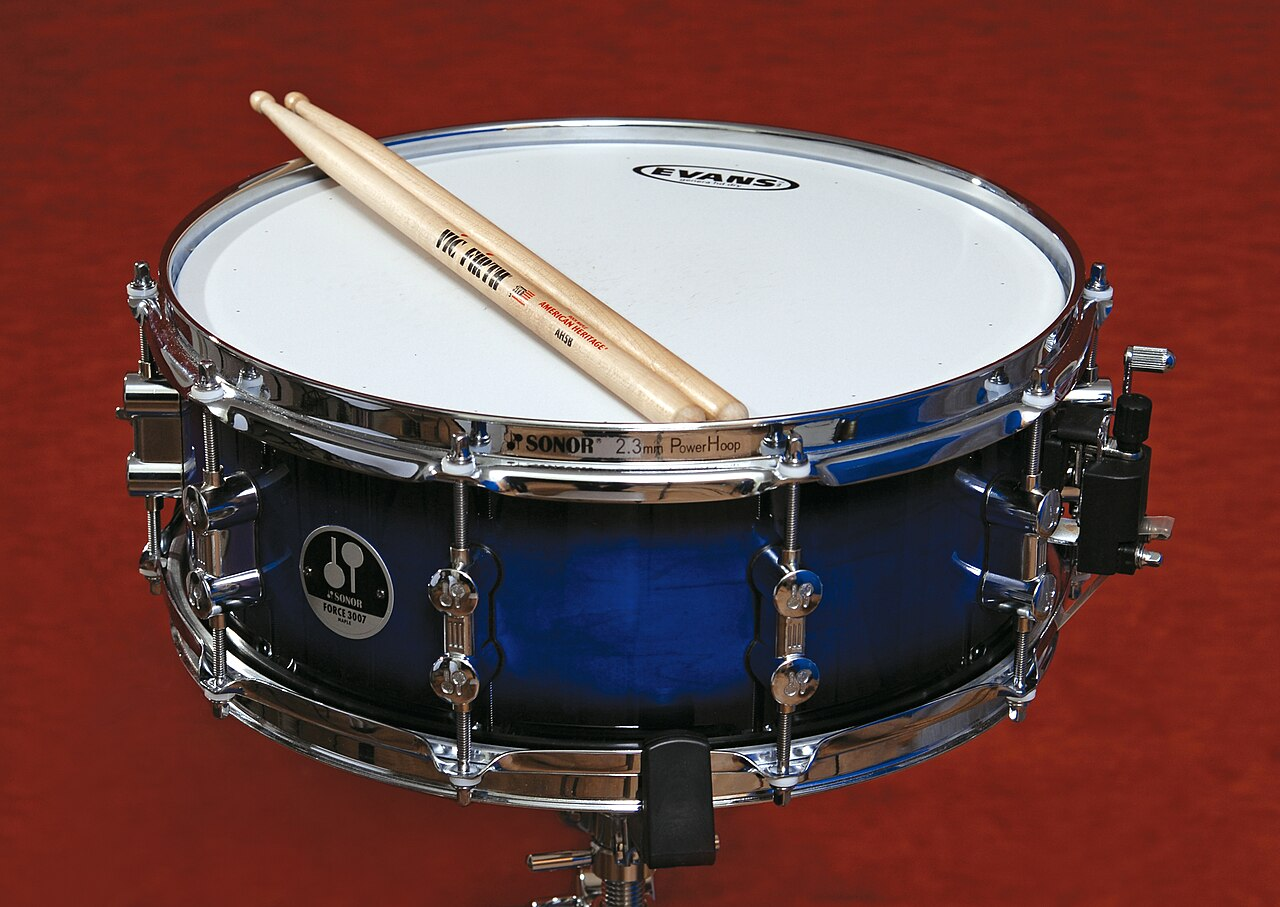
\includegraphics[width=0.58\linewidth]{images/book1/drum.jpg}

{\small Gendang sungguhan untuk percobaan beras: kulit putihnya adalah
bagian yang bergetar. Taburkan beberapa butir di atasnya, ketuk di
dekatnya --- kulit yang berbunyi adalah kulit yang bergetar, dan
berasnya menari untuk membuktikannya. \emph{Foto: Vladimir Morozov,
CC\ BY\ 2.0.}}
\end{omfigure}

\begin{proposition}[Tanpa getaran, tanpa bunyi]\label{prop:g3:sound-around-us:novib}
Setiap \omterm{def:g3:sound-around-us:sound}{bunyi} datang dari sebuah \omterm{def:g3:sound-around-us:vibration}{getaran} --- dan ketika \omterm{def:g3:sound-around-us:vibration}{getarannya}
berhenti, \omterm{def:g3:sound-around-us:sound}{bunyinya} pun berhenti seketika. Pukullah simbal dan biarkan
ia berdenting; lalu genggam erat-erat dengan kedua tangan: senyap,
begitu genggamanmu menghentikan getarnya.
\end{proposition}

\begin{example}[Sumber bunyi di mana-mana]\label{ex:g3:sound-around-us:sources}
Buruhlah \omterm{def:g3:sound-around-us:vibration}{getaran} di balik tiap \omterm{def:g3:sound-around-us:sound}{bunyi}: gitar --- senar yang dipetik
bergetar; gendang --- kulit yang dipukul bergetar; suaramu --- dua
lipatan kecil di tenggorokanmu bergetar ketika \omterm{def:g2:air-around-us:air}{udara} dari paru-parumu
menyembur melewatinya (itulah dengung yang tadi dirasakan jarimu);
lalat yang berdengung --- sayapnya bergetar ratusan kali tiap sekon;
pintu yang dibanting --- seluruh daun pintu dan kusennya bergidik
sesaat.
\end{example}

\section{Keras dan lirih, tinggi dan rendah}

\begin{example}[Keras berarti getaran yang lebar]\label{ex:g3:sound-around-us:loud}
Petiklah karet gelang yang teregang pelan-pelan: kabur yang kecil,
denting yang lirih. Petiklah kuat-kuat: kabur yang lebar, denting yang
keras. Makin kuat sumbernya bergetar --- makin lebar gerak
bolak-baliknya --- makin \emph{keras} \omterm{def:g3:sound-around-us:sound}{bunyinya}. Amati butiran berasnya
juga: ketukan yang lembut membuatnya bergidik, dentuman yang perkasa
melemparkannya ke \omterm{def:g2:air-around-us:air}{udara}.
\end{example}

\begin{example}[Tinggi dan rendah]\label{ex:g3:sound-around-us:pitch}
Regangkan karet gelang di atas kotak terbuka lalu petiklah; kemudian
jepit karetnya di tengah dan petiklah separuhnya yang pendek:
dentingnya menjadi \emph{lebih tinggi}, seperti cicit burung. Benda
yang pendek, tegang, dan tipis bergetar lebih cepat dan bernyanyi
tinggi; yang panjang, kendur, dan tebal bergetar lebih lambat dan
bernyanyi rendah. Itulah sebabnya seruling kecil mencicit dan tuba
besar menggeram --- dan mengapa senar gitar yang paling tipis
bernyanyi paling tinggi.
\end{example}

\begin{omfigure}
\begin{tikzpicture}[scale=0.85]
  % whole band, stretched over the open box, vibrating end to end
  \draw[thick] (0.3,0) rectangle (4.9,1.1);
  \draw[omDef, very thick] (0.3,1.1) -- (4.9,1.1);
  \draw[dashed, omDef] (0.3,1.1) .. controls (2.6,1.62) .. (4.9,1.1);
  \draw[dashed, omDef] (0.3,1.1) .. controls (2.6,0.58) .. (4.9,1.1);
  \node[below, font=\small, align=center] at (2.6,-0.3)
    {karet utuh:\\getaran lambat, denting rendah};
  % pinched at the middle: only the short half vibrates
  \draw[thick] (6.5,0) rectangle (11.1,1.1);
  \draw[omDef, very thick] (6.5,1.1) -- (11.1,1.1);
  \fill[omExo] (8.8,1.1) circle (0.1);
  \node[above, font=\footnotesize, omExo] at (8.8,1.32) {jepit};
  \draw[dashed, omDef] (8.8,1.1) .. controls (9.95,1.45) .. (11.1,1.1);
  \draw[dashed, omDef] (8.8,1.1) .. controls (9.95,0.75) .. (11.1,1.1);
  \node[below, font=\small, align=center] at (8.8,-0.3)
    {dijepit jadi pendek:\\getaran cepat, denting tinggi};
\end{tikzpicture}

{\small Gitar karet gelang: karet yang utuh berayun paling lebar di
tengahnya, tertambat pada kedua ujungnya, dan bernyanyi rendah;
separuhnya yang dijepit dan lebih pendek bergetar lebih cepat dan
bernyanyi lebih tinggi.}
\end{omfigure}

\begin{remark}[Jagalah gendang kecil di telingamu]\label{rem:g3:sound-around-us:ears}
Jauh di dalam telingamu, selaput mungil --- lebih tipis daripada
kertas --- bergetar bersama setiap \omterm{def:g3:sound-around-us:sound}{bunyi} yang datang, persis seperti
gendang berbutir beras tadi. \omterm{def:g3:sound-around-us:sound}{Bunyi} yang terlalu keras mengguncangnya
terlalu kuat: musik yang sangat keras, mesin, dan kembang api dapat
merusaknya untuk selamanya, dan selaput itu tidak tumbuh kembali.
Tutuplah telingamu di dekat kebisingan, dan jangan pernah berteriak ke
telinga siapa pun --- telinga tidak punya kelopak.
\end{remark}

\section{Dari sumber sampai ke telinga}

\begin{example}[Perjalanan sebuah tepukan]\label{ex:g3:sound-around-us:journey}
Seorang teman bertepuk di seberang halaman bermain. Tepukan itu
membuat \omterm{def:g2:air-around-us:air}{udara} bergetar; \omterm{def:g3:sound-around-us:vibration}{getarannya} menyebar melalui \omterm{def:g2:air-around-us:air}{udara} ke segala
arah, seperti riak di sekeliling kerikil yang dijatuhkan ke kolam;
sebagian \omterm{def:g3:sound-around-us:vibration}{getarannya} sampai ke telingamu dan membuat selaput kecil di
telingamu bergetar --- dan kamu mendengar tepukan itu. Sumber,
perjalanan, telinga: setiap \omterm{def:g3:sound-around-us:sound}{bunyi} yang pernah kamu dengar menempuh
perjalanan ini. Seberapa cepat perjalanannya, dan lewat apa saja ia
dapat merambat? Bab \omterm{def:g3:sound-around-us:sound}{bunyi} tahun depan mengambil persis kedua
pertanyaan itu.
\end{example}

\section{Latihan}

\begin{exercise}[$\star$]\label{exo:g3:sound-around-us:1}
Apa itu \omterm{def:g3:sound-around-us:vibration}{getaran}? Sebutkan bagian yang bergetar pada: gitar; \ gendang;
\ suaramu; \ lalat yang berdengung.
\end{exercise}

\begin{exercise}[$\star$]\label{exo:g3:sound-around-us:2}
Pada percobaan beras, apa yang dibuktikan oleh butiran yang melompat
tentang kulit gendang yang sedang berbunyi?
\end{exercise}

\begin{exercise}[$\star$]\label{exo:g3:sound-around-us:3}
Mengapa menggenggam simbal yang sedang berdenting membuatnya senyap
seketika? Hukum mana dalam bab ini yang sedang bekerja?
\end{exercise}

\begin{exercise}[$\star$]\label{exo:g3:sound-around-us:4}
Untuk membuat denting karet gelang \emph{lebih keras}, apa yang kamu
ubah pada petikanmu? Seperti apa kabur karetnya waktu itu?
\end{exercise}

\begin{exercise}[$\star$]\label{exo:g3:sound-around-us:5}
Mana yang bernyanyi lebih tinggi: karet pendek yang dijepit atau karet
yang utuh? \ Seruling kecil atau tuba besar? \ Senar gitar yang paling
tipis atau yang paling tebal?
\end{exercise}

\begin{exercise}[$\star$]\label{exo:g3:sound-around-us:6}
Berdendanglah dengan jarimu di tenggorokan, lalu berhentilah
mendendang. Apa yang dirasakan jarimu, dan tepat kapan rasa itu
berhenti?
\end{exercise}

\begin{exercise}[$\star$]\label{exo:g3:sound-around-us:7}
Ceritakan perjalanan sebuah tepukan dari tangan temanmu sampai ke
telingamu, dalam tiga langkah.
\end{exercise}

\begin{exercise}[$\star$]\label{exo:g3:sound-around-us:8}
Mengapa \omterm{def:g3:sound-around-us:sound}{bunyi} yang sangat keras harus dijauhkan dari telinga? Benda
mungil apa di dalam telinga yang terancam, dan ia mirip apa dalam bab
ini?
\end{exercise}

\begin{exercise}[$\star$]\label{exo:g3:sound-around-us:9}
Sisir sebuah kotak musik punya gigi dengan panjang berbeda-beda. Gigi
yang mana yang memainkan nada tinggi dan yang mana nada rendah?
Jawablah dengan aturan pada \cref{ex:g3:sound-around-us:pitch}.
\end{exercise}

\begin{exercise}[$\star\star$]\label{exo:g3:sound-around-us:10}
Tuangkan air ke dalam botol kaca lalu tiuplah melintasi mulutnya:
terdengar suitan! Tambahkan air lalu tiup lagi: suitannya menjadi
lebih tinggi. Apa yang bergetar sehingga terdengar suitan itu ---
kacanya, airnya, atau \omterm{def:g2:air-around-us:air}{udara} di dalamnya? Pakailah aturan
pendek-bernyanyi-tinggi untuk membela jawabanmu.
\end{exercise}

\begin{exercise}[$\star\star$]\label{exo:g3:sound-around-us:11}
Maya berkata: ``Ketika televisi dibisukan, gambarnya tetap bergerak
--- jadi gerakan saja pasti menghasilkan \omterm{def:g3:sound-around-us:sound}{bunyi}.'' Pakailah
\cref{def:g3:sound-around-us:sound} dan percobaan beras untuk
menjelaskan gerakan macam apa yang menghasilkan \omterm{def:g3:sound-around-us:sound}{bunyi}, dan mengapa
gambar di layar tidak menghasilkan \omterm{def:g3:sound-around-us:sound}{bunyi} sama sekali.
\end{exercise}
